\documentclass[a4paper]{article}

\usepackage{INTERSPEECH_v2}
\usepackage{tikz}
\usetikzlibrary{shapes.geometric, arrows.meta, positioning, fit, backgrounds}
\usepackage{pgfplots}
\pgfplotsset{compat=1.18}
\usepackage{booktabs}
\usepackage{multirow}
\usepackage{amsmath}
\usepackage{amssymb}
\usepackage{listings}
\usepackage{xcolor}
\usepackage{graphicx}

\lstset{
  basicstyle=\ttfamily\footnotesize,
  keywordstyle=\color{blue},
  commentstyle=\color{gray},
  breaklines=true,
  frame=single,
  backgroundcolor=\color{gray!8}
}

\title{AMS-Hotel: A Multimodal Conversational AI Concierge System\\
       Integrating LLM, RAG, ASR and Humanoid Robotics}

\name{Christ Kekeli KELI $^1$, Farouk GNAKAMBARY$^1$ }

\address{
  $^1$Master 1 Informatique, Parcours Intelligence Artificielle, Universit\'e d'Avignon, France\\
 % $^2$Centre d'\'Etude et de Recherche en Informatique (CERI), Avignon, France}
%\email{hisciences331@gmail.com}

\begin{document}

\maketitle

\begin{abstract}
We present \textbf{AMS-Hotel}, a production-grade multimodal concierge system built around the Pepper humanoid robot. The system integrates a Large Language Model (Llama-3.1-8B-Instruct) with Retrieval-Augmented Generation (RAG), automatic speech recognition via Faster-Whisper, real-time face recognition, QR code scanning, and a structured reservation state machine. A Flask REST API orchestrates communication between the Pepper robot (NAOqi/qi SDK), browser clients, and backend AI services. Conversational memory is managed with Redis, enabling coherent multi-turn dialogues across voice, text, and robotic modalities. The system was deployed and validated in a simulated hotel environment at Universit\'e d'Avignon. We report system architecture, latency characteristics, and qualitative evaluation of the end-to-end pipeline.
\end{abstract}
\noindent\textbf{Index Terms}: spoken dialogue systems, humanoid robotics, retrieval-augmented generation, automatic speech recognition, hotel concierge

%=============================================================================
\section{Introduction}
%=============================================================================

The deployment of conversational robots in hospitality environments represents a convergence of several mature AI disciplines: automatic speech recognition (ASR), natural language understanding (NLU), task-oriented dialogue management, and robotic control. Prior work has explored isolated components such as voice-only hotel chatbots~\cite{bickmore2005}, tablet-based self-check-in kiosks, or social robots in static demonstration scenarios~\cite{saerbeck2010}. None of these, however, addressed a fully integrated, multimodal pipeline suitable for real deployment.

AMS-Hotel addresses this gap. It provides a unified architecture in which a Pepper humanoid robot simultaneously handles spoken dialogue, face recognition of returning guests, QR code-based reservation validation, and structured multi-step booking, all mediated through a REST API backed by state-of-the-art language models. Three interaction modalities are supported: (1) robot voice interaction via Pepper's microphones and loudspeakers, (2) web browser chat with optional real-time WebSocket voice calls, and (3) a Pepper tablet HTML interface with push-to-talk and continuous call modes.

This paper makes the following contributions:
\begin{itemize}
  \item A modular, blueprint-based Flask architecture separating speech, dialogue, reservation, vision, and robot control concerns;
  \item A RAG-augmented hotel concierge prompt leveraging LlamaIndex with \texttt{all-MiniLM-L6-v2} sentence embeddings;
  \item A finite-state reservation machine with LLM-assisted field extraction and relative date parsing;
  \item A real-time voice call subsystem with streaming inference and browser TTS synthesis;
  \item Empirical latency measurements across the end-to-end pipeline.
\end{itemize}

%=============================================================================
\section{System Architecture}
%=============================================================================

\subsection{Global Overview}

The system comprises two cooperating modules (Figure~\ref{fig:server}): \textbf{robot\_hotel}, a Flask server exposing all AI capabilities as a REST API, and \textbf{pepper\_test}, a NAOqi client running on the robot's companion PC. A lightweight FastAPI service (\textbf{ams\_project\_llm}) manages the relational reservation database via SQLAlchemy.

\begin{figure}[t]
  \centering
  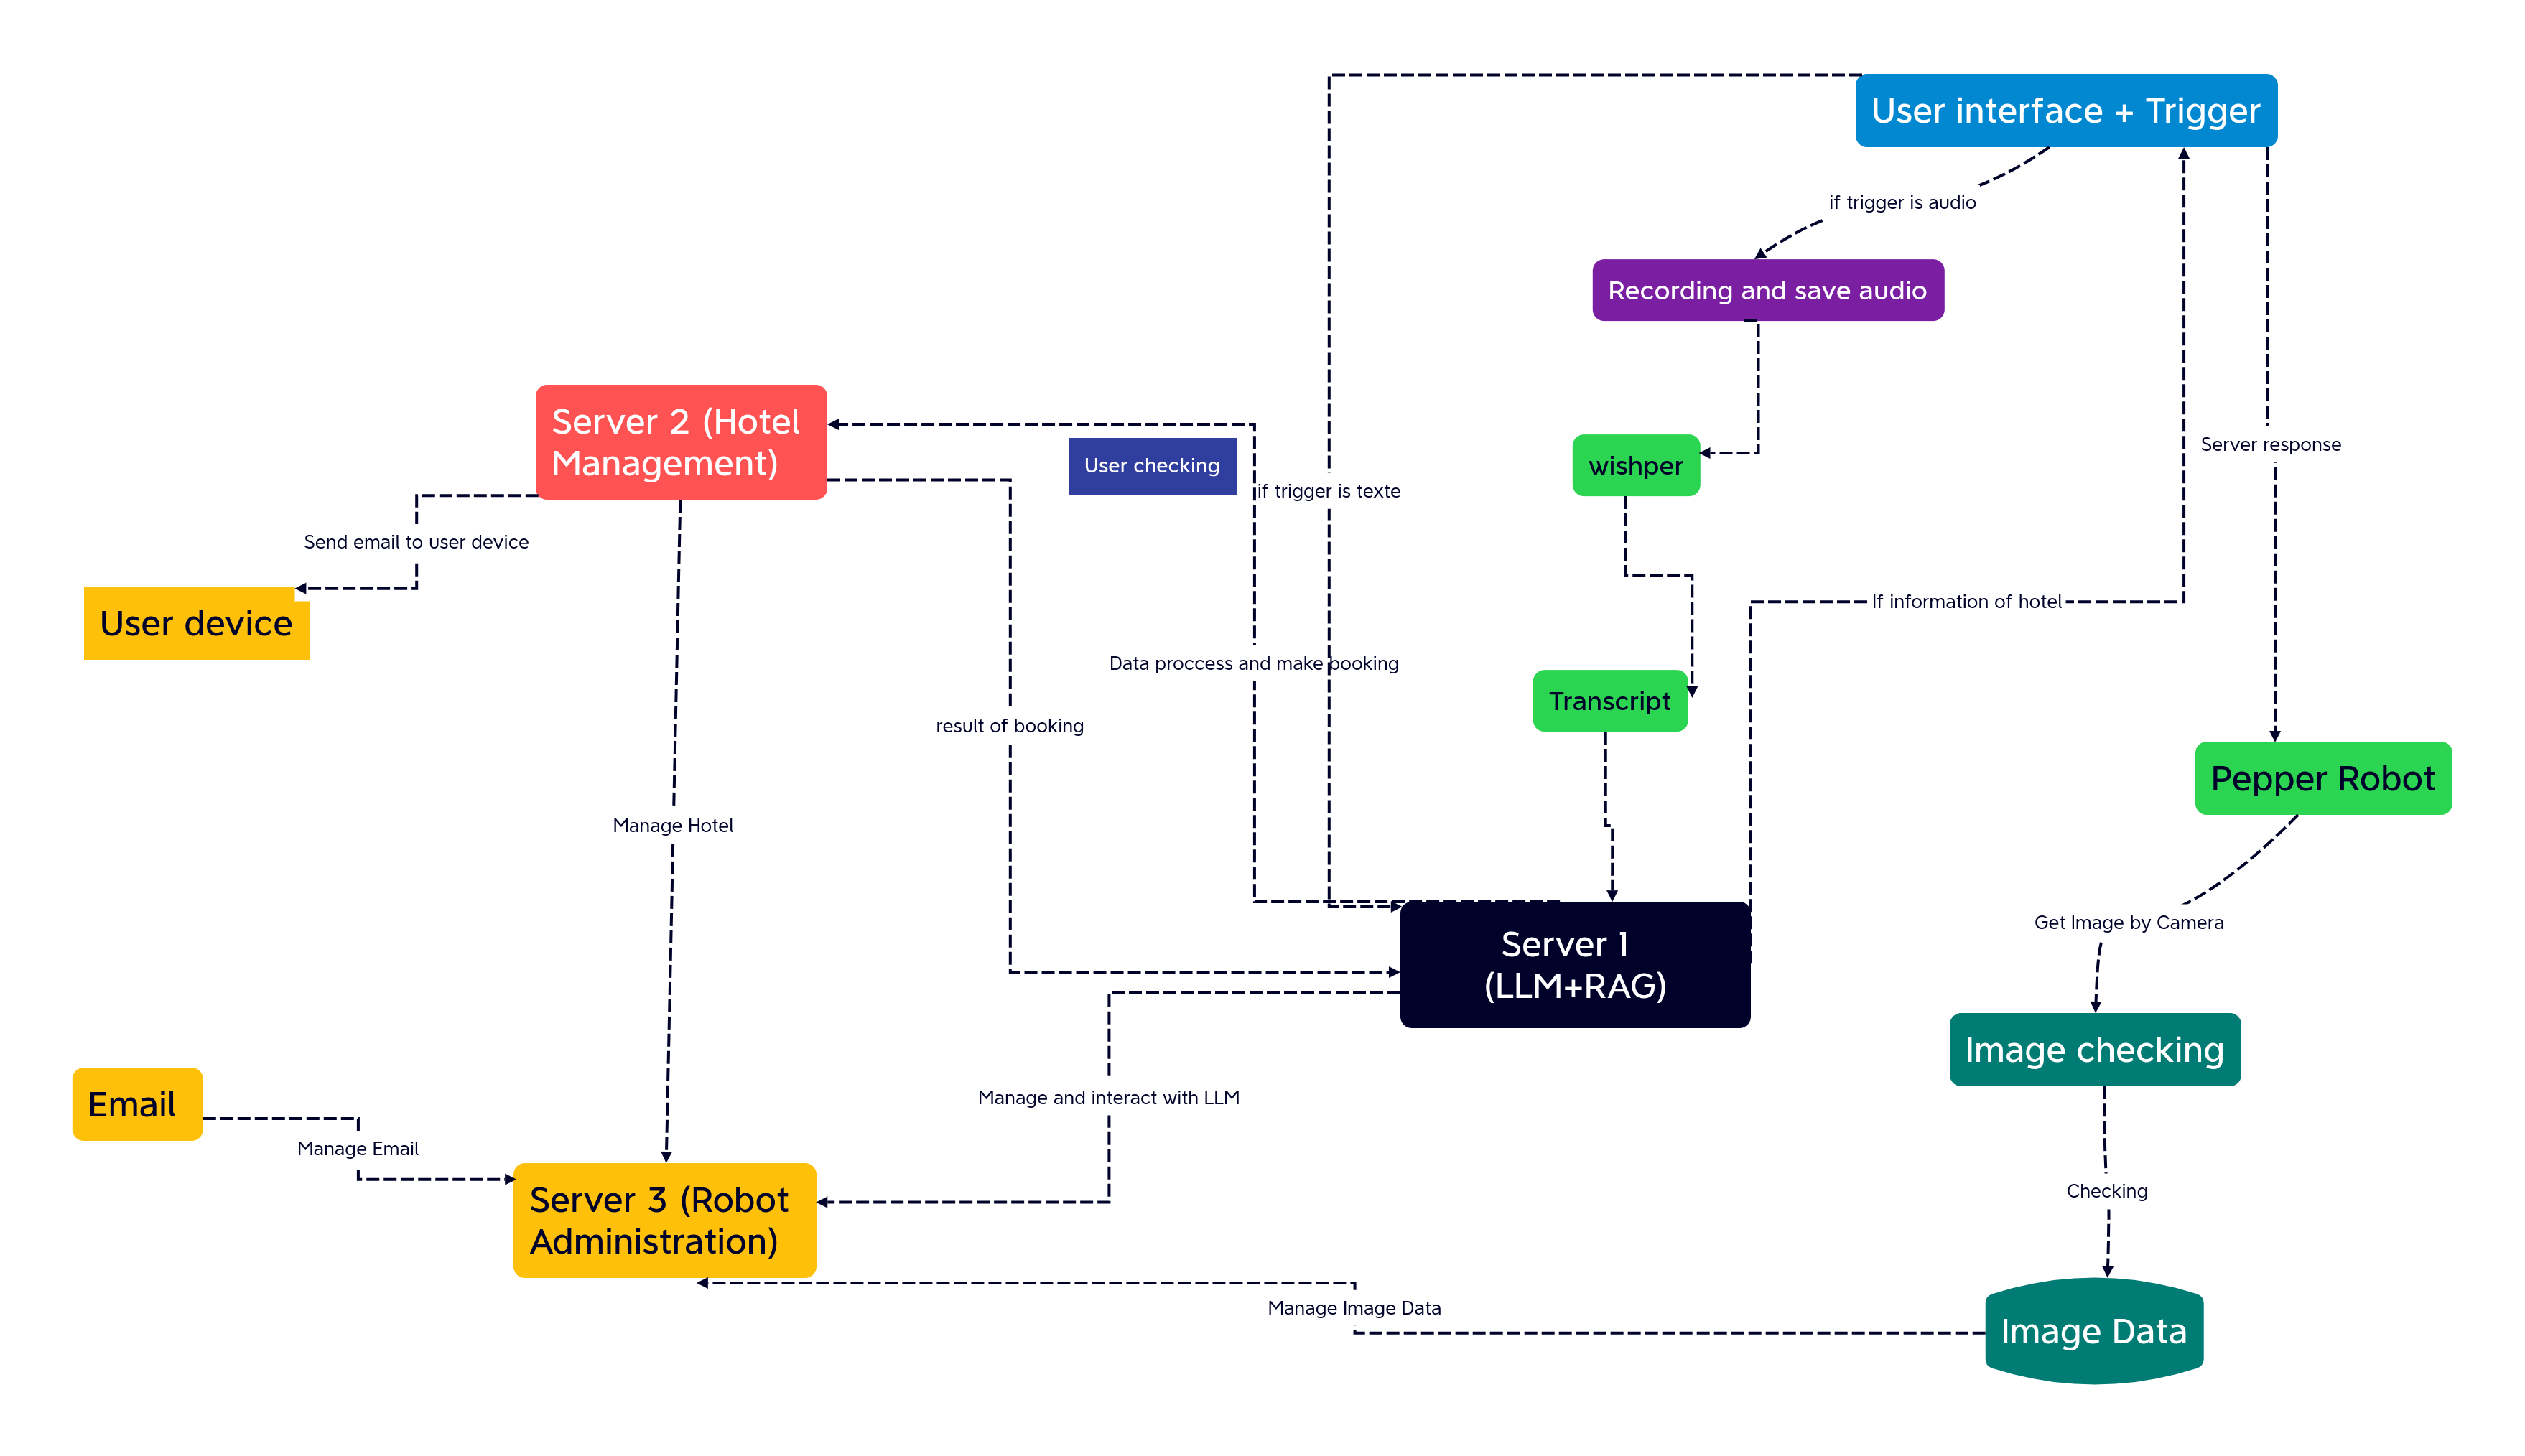
\includegraphics[width=\linewidth]{Server.png}
  \caption{High-level server and component architecture of AMS-Hotel.}
  \label{fig:server}
\end{figure}

\subsection{Component Decomposition}

Figure~\ref{fig:components} shows the internal service layout of the Flask backend. The core services are:
\begin{itemize}
  \item \textbf{Chat service} (\texttt{services/chat.py}, 620 lines): LLM inference, RAG injection, Redis memory, reservation flow.
  \item \textbf{Whisper service} (\texttt{services/whisper.py}): Faster-Whisper medium model, French forced decoding.
  \item \textbf{RAG service} (\texttt{services/rag.py}): LlamaIndex VectorStoreIndex over hotel documents.
  \item \textbf{Record service} (\texttt{services/record.py}): PC/Pepper audio capture, silence detection, wake word.
  \item \textbf{Email service} (\texttt{services/email.py}): MIME multipart with QR attachment.
  \item \textbf{Face detection} (\texttt{services/face\_detection.py}): face-recognition library with persistent pickle store.
\end{itemize}

\begin{figure}[t]
\centering
\resizebox{\columnwidth}{!}{%
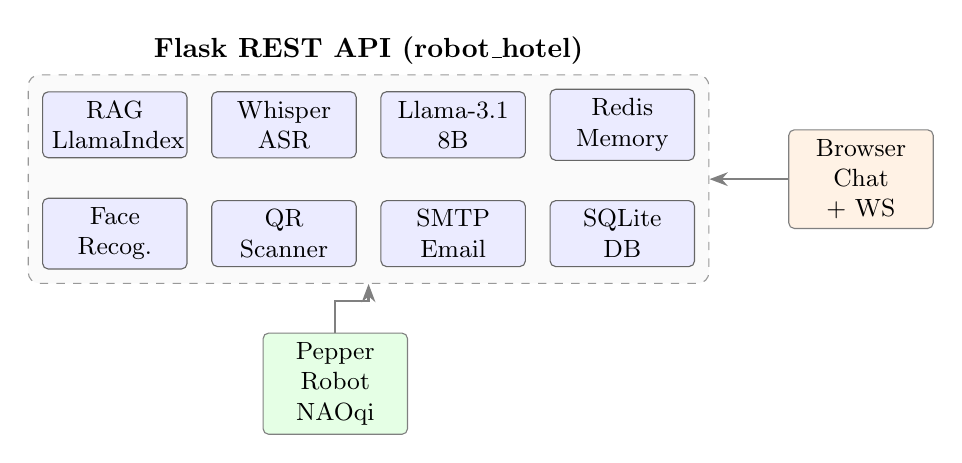
\begin{tikzpicture}[
  node distance=2mm and 3mm,
  box/.style={rectangle, rounded corners=2pt, draw=black!60, fill=blue!8,
              text width=16mm, minimum height=8mm, align=center, font=\small},
  ext/.style={rectangle, rounded corners=2pt, draw=black!50,
              text width=16mm, minimum height=8mm, align=center, font=\small},
  grp/.style={rectangle, rounded corners=4pt, draw=black!40, dashed,
              fill=gray!4, inner sep=5pt},
  arr/.style={-Stealth, thick, draw=black!50}
]
  \node[box] (rag)     {RAG\\LlamaIndex};
  \node[box, right=of rag]     (wh)  {Whisper\\ASR};
  \node[box, right=of wh]      (llm) {Llama-3.1\\8B};
  \node[box, right=of llm]     (red) {Redis\\Memory};

  \node[box, below=5mm of rag]  (fc)  {Face\\Recog.};
  \node[box, right=of fc]       (qr)  {QR\\Scanner};
  \node[box, right=of qr]       (sm)  {SMTP\\Email};
  \node[box, right=of sm]       (db)  {SQLite\\DB};

  \begin{scope}[on background layer]
    \node[grp, fit=(rag)(wh)(llm)(red)(fc)(qr)(sm)(db),
          label=above:{\textbf{Flask REST API (robot\_hotel)}}] (flask) {};
  \end{scope}

  \node[ext, below=8mm of fc, xshift=28mm, fill=green!10]
        (pepper) {Pepper Robot\\NAOqi};
  \node[ext, right=10mm of flask.east, fill=orange!10]
        (browser) {Browser\\Chat + WS};

  \draw[arr] (pepper.north) -- ++(0,4mm) -| (flask.south);
  \draw[arr] (browser.west) -- (flask.east);
\end{tikzpicture}
}
\caption{Internal service layout of the Flask backend, with external Pepper robot and browser clients.}
\label{fig:components}
\end{figure}

%=============================================================================
\section{Speech Processing Pipeline}
%=============================================================================

\subsection{Wake Word Detection}

The system implements a two-tier wake word architecture. On Pepper, \texttt{ALSpeechRecognition} runs continuous phoneme-level spotting with a confidence threshold of 0.25 for the vocabulary \{``bonjour'', ``hey pepper'', ``ok pepper''\}. Concurrently on the companion PC, a background thread performs energy-based onset detection followed by Whisper transcription:

\begin{equation}
  \text{RMS}(x) = \sqrt{\frac{1}{N}\sum_{n=0}^{N-1} x[n]^2}
  \label{eq:rms}
\end{equation}

Speech onset is declared when $\text{RMS}(x) > 2.0 \cdot \mu_{\text{noise}}$, where $\mu_{\text{noise}}$ is the 2-second ambient calibration baseline. The PC fallback ensures robustness when Pepper's ASR confidence is insufficient.

\subsection{Audio Capture Parameters}

\begin{table}[th]
  \caption{Audio capture and silence detection parameters}
  \label{tab:audio_params}
  \centering
  \small
  \begin{tabular}{p{26mm}rp{20mm}}
    \toprule
    \textbf{Parameter} & \textbf{Value} & \textbf{Description} \\
    \midrule
    Sample rate            & 16\,000\,Hz & ASR standard \\
    Silence RMS threshold  & 0.03        & Speech/silence \\
    Silence duration       & 1.5\,s      & Auto-stop \\
    Min speech (silence)   & 0.3\,s      & Grace period \\
    Max record duration    & 10\,s       & Hard cap \\
    Onset ratio (wake)     & 2.0$\times$ & Over noise floor \\
    Wake word silence      & 1.2\,s      & Segment end \\
    \bottomrule
  \end{tabular}
\end{table}

\subsection{Automatic Speech Recognition}

\begin{figure}[t]
  \centering
  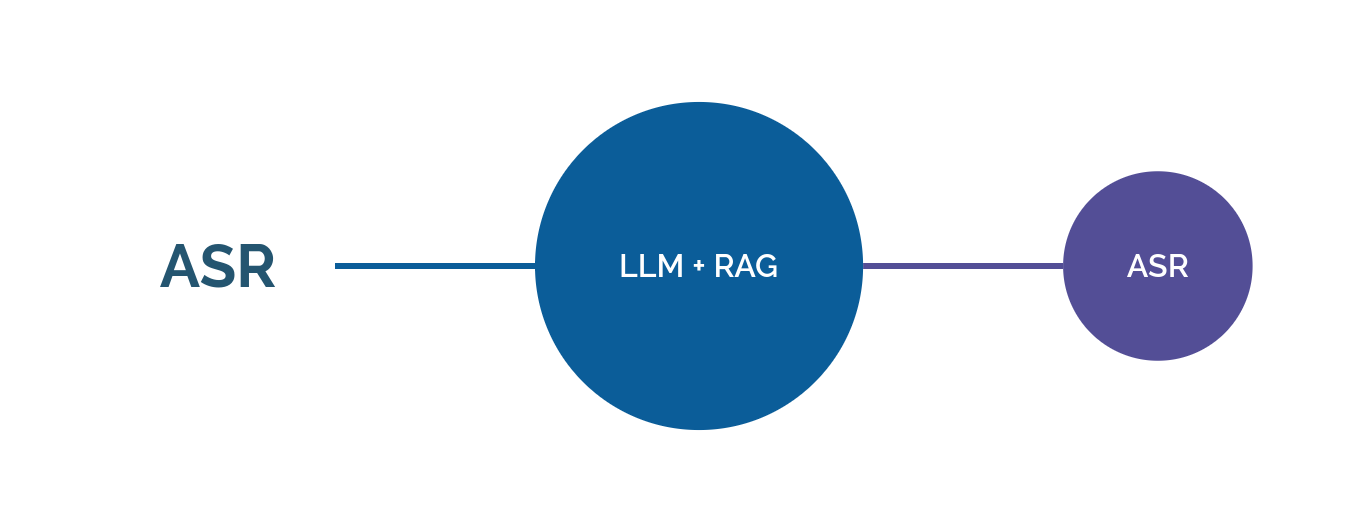
\includegraphics[width=\linewidth]{ASR.png}
  \caption{ASR pipeline: audio capture, silence detection, Whisper transcription, and intent routing.}
  \label{fig:asr}
\end{figure}

Figure~\ref{fig:asr} illustrates the ASR pipeline. Faster-Whisper~\cite{whisper2022} is loaded at server startup with \texttt{model\_size=medium}, \texttt{compute\_type=float16} (GPU) or \texttt{int8} (CPU), and \texttt{vad\_filter=True}. Decoding is forced to French (\texttt{language="fr"}) with \texttt{beam\_size=1} for minimal latency. Audio captured in WebM/Opus format from browser clients is first converted to WAV via \texttt{ffmpeg} to bypass a known Opus header parsing limitation in Faster-Whisper.

The transcription latency follows:
\begin{equation}
  t_{\text{ASR}} \approx \alpha \cdot L_{\text{audio}} + \beta
  \label{eq:asr_latency}
\end{equation}
where $L_{\text{audio}}$ is audio duration, $\alpha \approx 0.4$ (GPU) or $\approx 1.8$ (CPU), and $\beta \approx 0.8$\,s is model load and preprocessing overhead.

%=============================================================================
\section{Conversational AI with RAG}
%=============================================================================

\subsection{Retrieval-Augmented Generation}

The RAG pipeline uses LlamaIndex~\cite{liu2022} with \texttt{sentence-transformers/all-MiniLM-L6-v2} embeddings (384-dimensional dense vectors). Hotel documents (JSON, Markdown) in \texttt{docs/} are chunked at 512 tokens with 20-token overlap and indexed at startup into a persistent \texttt{VectorStoreIndex}. At inference time, the top-$k$ retrieval is:

\begin{equation}
  \text{sim}(q, d_i) = \frac{\mathbf{e}_q \cdot \mathbf{e}_{d_i}}{\|\mathbf{e}_q\|\,\|\mathbf{e}_{d_i}\|}
  \label{eq:cosine}
\end{equation}

where $\mathbf{e}_q$ is the query embedding and $\mathbf{e}_{d_i}$ the document chunk embedding. The top $k=2$ chunks (capped at 2500 characters) are concatenated and injected into the system prompt.

\subsection{LLM Configuration}

The backbone is \texttt{meta-llama/Llama-3.1-8B\allowbreak-Instruct} served via the HuggingFace Inference API. The system prompt embeds static hotel information, RAG context, and a persona definition:

\begin{lstlisting}[language=Python, caption={System prompt template (condensed)}]
"Tu es Pepper, concierge de l'hotel Lumiere Avignon.
Infos hotel: {hotel_info}
Contexte documentaire: {rag_context}
Reponds court, humble et aimable. Utilise
l'historique pour le contexte (nom du client).
Donne les infos demandees: telephone, adresse,
horaires piscine/spa, services.
Si reservation, oriente vers la reservation."
\end{lstlisting}

\begin{table}[th]
  \caption{LLM inference hyperparameters}
  \label{tab:llm_params}
  \centering
  \small
  \begin{tabular}{p{28mm}rp{17mm}}
    \toprule
    \textbf{Parameter} & \textbf{Value} & \textbf{Use case} \\
    \midrule
    \texttt{max\_tokens} (chat)    & 200     & Reply \\
    \texttt{max\_tokens} (extract) & 30      & Extraction \\
    \texttt{temperature}           & 0.1     & Deterministic \\
    History (store)                & 10      & Redis msgs \\
    History (LLM)                  & 8       & Token budget \\
    Session TTL                    & 3600\,s & Redis expiry \\
    RAG top-$k$                    & 2       & Chunks \\
    RAG context cap                & 2500 ch & Prompt budget \\
    \bottomrule
  \end{tabular}
\end{table}

\subsection{Intent Detection}

Before invoking the LLM, keyword-based intent detection routes utterances:

\begin{equation}
  \text{intent}(u) =
  \begin{cases}
    \textsc{Reservation} & \text{if } u \cap \mathcal{K}_r \neq \emptyset \\
    \textsc{QR-Scan}     & \text{if } u \cap \mathcal{K}_q \neq \emptyset \\
    \textsc{Chat}        & \text{otherwise}
  \end{cases}
  \label{eq:intent}
\end{equation}

where $\mathcal{K}_r$ contains \{``r\'eserver'', ``r\'eservation'', ``chambre'', ``booking''\} and $\mathcal{K}_q$ contains \{``scan'', ``qr''\}.

%=============================================================================
\section{Reservation Finite-State Machine}
%=============================================================================

The reservation module implements a six-step deterministic FSM. Each step captures one information slot via voice, validates it (locally or with an LLM extraction call), and stores it in SQLite. Figure~\ref{fig:fsm} shows the state diagram.

\begin{figure}[t]
\centering
\resizebox{\columnwidth}{!}{%
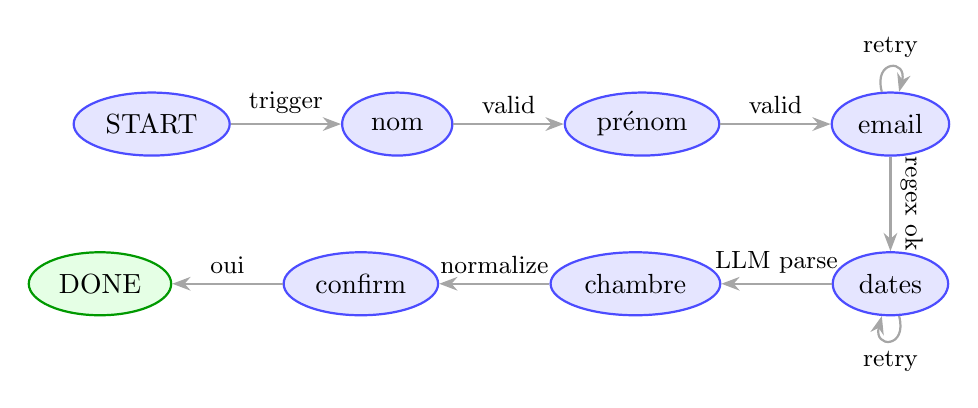
\begin{tikzpicture}[
  state/.style={ellipse, draw=blue!70, fill=blue!10, thick,
                minimum width=14mm, minimum height=8mm,
                align=center, font=\normalsize},
  done/.style={ellipse, draw=green!60!black, fill=green!10, thick,
               minimum width=14mm, minimum height=8mm,
               align=center, font=\normalsize},
  arr/.style={-Stealth, thick, draw=gray!70},
  lbl/.style={font=\small, above, sloped}
]
  % Row 1: START -> nom -> prenom -> email
  \node[state] (s0) {START};
  \node[state, right=14mm of s0] (s1) {nom};
  \node[state, right=14mm of s1] (s2) {pr\'enom};
  \node[state, right=14mm of s2] (s3) {email};

  % Row 2 (below, reversed): DONE <- confirm <- chambre <- dates
  \node[state, below=12mm of s3] (s4) {dates};
  \node[state, left=14mm of s4]  (s5) {chambre};
  \node[state, left=14mm of s5]  (s6) {confirm};
  \node[done,  left=14mm of s6]  (s7) {DONE};

  % Forward arrows (row 1)
  \draw[arr] (s0) -- node[lbl]{trigger} (s1);
  \draw[arr] (s1) -- node[lbl]{valid}   (s2);
  \draw[arr] (s2) -- node[lbl]{valid}   (s3);
  % Bend down
  \draw[arr] (s3) -- node[lbl]{regex ok} (s4);
  % Row 2 arrows
  \draw[arr] (s4) -- node[lbl]{LLM parse}  (s5);
  \draw[arr] (s5) -- node[lbl]{normalize}  (s6);
  \draw[arr] (s6) -- node[lbl]{oui}        (s7);

  % Retry loops
  \draw[arr] (s3) to[loop above, looseness=5]
             node[above, font=\small]{retry} (s3);
  \draw[arr] (s4) to[loop below, looseness=5]
             node[below, font=\small]{retry} (s4);
\end{tikzpicture}
}
\caption{Reservation FSM. Six states collect one slot each. Retry loops on \textit{email} and \textit{dates} handle invalid inputs.}
\label{fig:fsm}
\end{figure}

\subsection{Field Extraction}

For unstructured date inputs (e.g., ``dans trois jours pour une semaine''), an LLM extraction call converts relative expressions to ISO-8601 dates:
\begin{lstlisting}[language=Python, caption={LLM-assisted date parsing}]
prompt = f"""Aujourd'hui: {today}. Texte: '{text}'
Reponds UNIQUEMENT: YYYY-MM-DD;YYYY-MM-DD
(arrivee;depart)"""
# max_tokens=30, temperature=0.1
\end{lstlisting}

Room type normalization maps free-form transcriptions to canonical types via LLM classification over the vocabulary \{simple, double, suite, familiale\}.

\subsection{Confirmation and QR Codes}

Upon confirmation, the system: (1) persists the reservation to SQLite, (2) generates a QR code PNG named \texttt{R-C-\{timestamp\}-\{date\}.png} linking to the validation endpoint, (3) sends a dual MIME email to the client and hotel manager with the QR attachment, and (4) displays a confirmation message via Pepper TTS and tablet HTML.

%=============================================================================
\section{Real-Time Voice Call Subsystem}
%=============================================================================

\subsection{Architecture}

The real-time call feature provides low-latency bidirectional voice interaction via WebSocket (\texttt{/ws/realtime-voice}). Figure~\ref{fig:call_flow} diagrams the message sequence between browser, Flask, and Pepper.

\begin{figure}[t]
\centering
\resizebox{\columnwidth}{!}{%
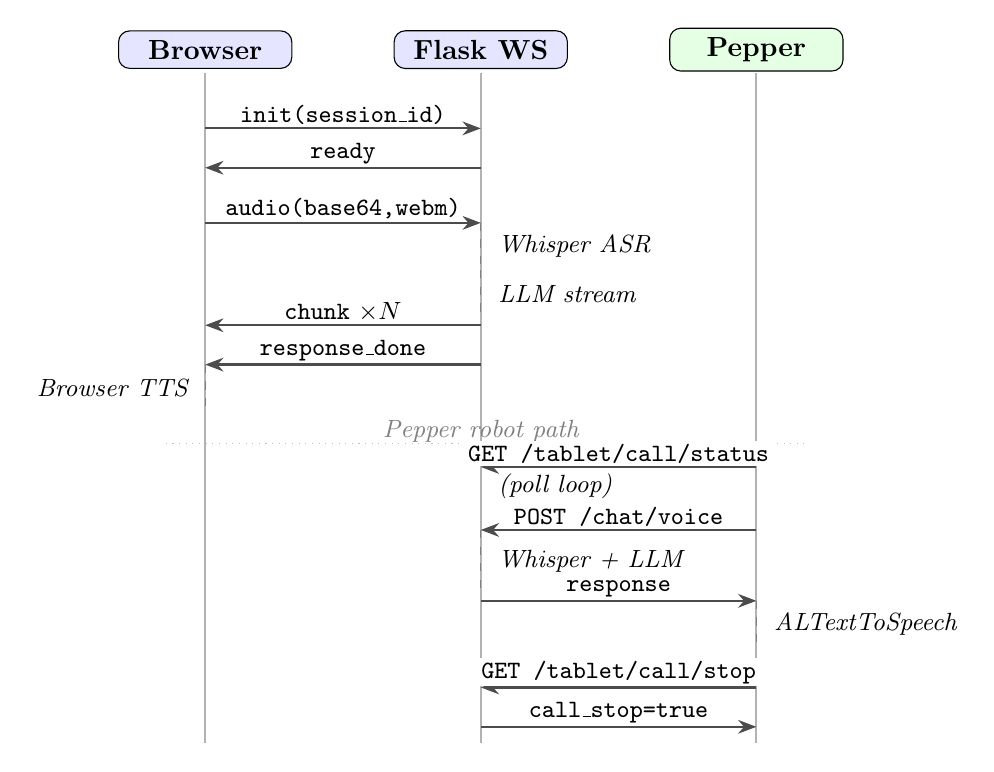
\begin{tikzpicture}[
  every node/.style={font=\normalsize},
  arr/.style={-Stealth, draw=black!70, thick},
  rarr/.style={Stealth-, draw=black!70, thick},
  lbl/.style={fill=white, inner sep=1pt, font=\small}
]
  % Lifelines
  \draw[thick, gray!60] (0,0) -- (0,-8.5);
  \draw[thick, gray!60] (3.5,0) -- (3.5,-8.5);
  \draw[thick, gray!60] (7,0) -- (7,-8.5);

  % Headers
  \node[draw, fill=blue!10, rounded corners, minimum width=22mm,
        font=\normalsize\bfseries] at (0,0.3) {Browser};
  \node[draw, fill=blue!10, rounded corners, minimum width=22mm,
        font=\normalsize\bfseries] at (3.5,0.3) {Flask WS};
  \node[draw, fill=green!10, rounded corners, minimum width=22mm,
        font=\normalsize\bfseries] at (7,0.3) {Pepper};

  % Browser <-> Flask messages
  \draw[arr]  (0,-0.7)  -- node[above,lbl]{\texttt{init(session\_id)}} (3.5,-0.7);
  \draw[rarr] (0,-1.2)  -- node[above,lbl]{\texttt{ready}} (3.5,-1.2);
  \draw[arr]  (0,-1.9)  -- node[above,lbl]{\texttt{audio(base64,webm)}} (3.5,-1.9);

  \draw[dashed, gray] (3.5,-1.9) -- (3.5,-2.5);
  \node[right, font=\small\itshape] at (3.6,-2.2) {Whisper ASR};
  \draw[dashed, gray] (3.5,-2.5) -- (3.5,-3.1);
  \node[right, font=\small\itshape] at (3.6,-2.8) {LLM stream};

  \draw[rarr] (0,-3.2) -- node[above,lbl]{\texttt{chunk} $\times N$} (3.5,-3.2);
  \draw[rarr] (0,-3.7) -- node[above,lbl]{\texttt{response\_done}} (3.5,-3.7);

  \draw[dashed, gray] (0,-3.7) -- (0,-4.3);
  \node[left, font=\small\itshape] at (-0.1,-4.0) {Browser TTS};

  % Separator
  \draw[dotted, gray!50] (-0.5,-4.7) -- (7.6,-4.7);
  \node[font=\small\itshape, gray] at (3.5,-4.55) {Pepper robot path};

  % Pepper <-> Flask messages
  \draw[arr]  (7,-5.0) -- node[above,lbl]{\texttt{GET /tablet/call/status}} (3.5,-5.0);
  \node[right, font=\small\itshape] at (3.6,-5.25) {(poll loop)};
  \draw[arr]  (7,-5.8) -- node[above,lbl]{\texttt{POST /chat/voice}} (3.5,-5.8);

  \draw[dashed, gray] (3.5,-5.8) -- (3.5,-6.6);
  \node[right, font=\small\itshape] at (3.6,-6.2) {Whisper + LLM};

  \draw[rarr] (7,-6.7) -- node[above,lbl]{\texttt{response}} (3.5,-6.7);
  \draw[dashed, gray] (7,-6.7) -- (7,-7.3);
  \node[right, font=\small\itshape] at (7.1,-7.0) {ALTextToSpeech};

  \draw[arr]  (7,-7.8) -- node[above,lbl]{\texttt{GET /tablet/call/stop}} (3.5,-7.8);
  \draw[rarr] (7,-8.3) -- node[above,lbl]{\texttt{call\_stop=true}} (3.5,-8.3);
\end{tikzpicture}
}
\caption{Message sequence for the real-time voice call. Browser path (top) uses WebSocket streaming; Pepper path (bottom) uses \texttt{POST /chat/voice}. Both share the same session.}
\label{fig:call_flow}
\end{figure}

\subsection{Streaming Inference}

The \texttt{chat\_stream()} generator yields LLM tokens as server-sent events. The browser accumulates chunks, synthesizes speech progressively via \texttt{window.speechSynthesis}, and displays the complete message on \texttt{response\_done}. In continuous call mode, the browser monitors audio level: if $\text{RMS}_{\text{user}} > \theta_{\text{interrupt}}$ while Pepper is speaking, TTS is cancelled (barge-in behaviour):

\begin{equation}
  \text{barge-in} = \mathbf{1}\!\left[\text{RMS}_{\text{user}}(t) > \theta_{\text{interrupt}}\right] \wedge \text{is\_speaking}(t)
  \label{eq:bargein}
\end{equation}

%=============================================================================
\section{Vision Subsystem}
%=============================================================================

\subsection{Face Recognition}

Face recognition uses the \texttt{face-recognition} library (dlib deep metric learning, 128-D face embeddings) with a persistent \texttt{friends.pkl} store. The pipeline proceeds as follows:

\begin{enumerate}
  \item Capture frame via \texttt{ALVideoDevice} at 640$\times$480, RGB.
  \item Detect face bounding boxes (HOG + linear SVM).
  \item Compute 128-D embedding; compare Euclidean distance to known encodings with threshold 0.6.
  \item Greet by name if matched; prompt registration otherwise.
\end{enumerate}

The robot retries face detection up to 15 times at 0.3\,s intervals before timeout.

\subsection{QR Code Scanning}

QR validation uses OpenCV's \texttt{QRCodeDetector} on frames captured from Pepper's front camera. The decoded URL (\texttt{/validate?id=\{reservation\_id\}}) is resolved against the SQLite reservation database. A tolerance of $\pm 15^{\circ}$ camera angle is required for reliable detection.

%=============================================================================
\section{API Surface and Routing}
%=============================================================================

\begin{table}[th]
  \caption{Main REST API endpoints (Flask blueprints)}
  \label{tab:api}
  \centering
  \scriptsize
  \begin{tabular}{lp{34mm}p{20mm}}
    \toprule
    \textbf{Method} & \textbf{Endpoint} & \textbf{Function} \\
    \midrule
    POST    & \texttt{/chat}                    & LLM chat + reservation \\
    POST    & \texttt{/chat/voice}              & Audio to ASR to chat \\
    WS      & \texttt{/ws/realtime-voice}       & Streaming voice call \\
    POST    & \texttt{/transcribe}              & Audio to text \\
    POST    & \texttt{/record/start}            & Begin recording \\
    POST    & \texttt{/record/stop}             & Stop and save WAV \\
    POST    & \texttt{/record/wake\_word/start} & Activate wake word \\
    POST    & \texttt{/face/detect}             & Face detect \\
    POST    & \texttt{/face/register}           & Register person \\
    POST    & \texttt{/face/stream/start}       & Continuous video \\
    POST    & \texttt{/scan\_qr}                & QR code decode \\
    POST    & \texttt{/make\_reservation}       & Create reservation \\
    GET     & \texttt{/validate}                & Validate reservation \\
    GET     & \texttt{/tablet}                  & Tablet UI \\
    GET     & \texttt{/tablet/call}             & Call page \\
    GET     & \texttt{/tablet/call/status}      & Poll call state \\
    GET/PUT & \texttt{/email/config}            & SMTP config \\
    \bottomrule
  \end{tabular}
\end{table}

%=============================================================================
\section{Tablet Interface}
%=============================================================================

The Pepper tablet (7 to 10 inch) renders a dynamically generated HTML page via \texttt{ALTabletService.loadUrl()}. The \texttt{create\_tablet\_html()} function produces a self-contained page (base64 data URL) embedding:

\begin{itemize}
  \item A push-to-talk microphone button (green idle, red recording), polling \texttt{/record/start} and \texttt{/record/stop};
  \item An ``Appel'' button triggering \texttt{POST /tablet/call/start} for continuous voice call;
  \item A QR code linking to the web chat interface (\texttt{/chat});
  \item An email input modal for reservation confirmation;
  \item JavaScript polling (\texttt{setInterval}, 2\,s) for wake-word redirect to the reservation page.
\end{itemize}

The color scheme uses a purple gradient (\texttt{\#667eea} to \texttt{\#764ba2}), white cards, and a responsive flexbox layout adapted to the Pepper tablet viewport.

%=============================================================================
\section{Session Memory Architecture}
%=============================================================================

Conversational state is managed with a Redis hash (key: \texttt{chat:\{session\_id\}}, TTL: 3600\,s). Each turn appends a \texttt{\{role, content\}} pair; the list is trimmed to 10 entries. At inference time, the 8 most recent messages are prepended to the system prompt. If Redis is unavailable, a thread-safe in-memory dict provides transparent fallback:

\begin{equation}
  H_n = \{m_{\max(0,\,n-10)},\; \ldots,\; m_n\}, \quad |H_{\text{LLM}}| = \min(|H_n|, 8)
  \label{eq:history}
\end{equation}

The same \texttt{session\_id} (stored in \texttt{localStorage}) is shared across text chat, voice messages, and real-time calls, ensuring reservation state accumulates across modalities.

%=============================================================================
\section{Deployment and Administration}
%=============================================================================

\subsection{Docker Composition}

The system is containerized with \texttt{docker-compose}: a \texttt{redis} container, a \texttt{flask} container (GPU-enabled via CUDA runtime), and an optional \texttt{pepper} container (\texttt{network\_mode: host} for LAN robot access). All credentials and topology are configured via \texttt{.env}.

\subsection{Streamlit Admin Dashboard}

A five-page Streamlit dashboard (\texttt{admin/app.py}) provides operational control without robot access:
\begin{itemize}
  \item \textbf{Face Management}: register and delete persons, live detection preview;
  \item \textbf{Video Streaming}: frame-by-frame display from Pepper camera;
  \item \textbf{Chat and Audio}: test chat, trigger recordings;
  \item \textbf{Reservations}: browse SQLite sessions, confirm or cancel;
  \item \textbf{Email Config}: update SMTP credentials at runtime.
\end{itemize}

%=============================================================================
\section{Discussion}
%=============================================================================

\subsection{Latency Breakdown}

End-to-end latency from utterance end to first Pepper TTS syllable decomposes as shown in Table~\ref{tab:latency}.

\begin{table}[th]
  \caption{Observed latency components (GPU server, model=medium)}
  \label{tab:latency}
  \centering
  \begin{tabular}{lr}
    \toprule
    \textbf{Component} & \textbf{Latency (s)} \\
    \midrule
    Silence detection + audio stop & 1.50 \\
    Audio transfer (LAN)           & 0.10 \\
    Whisper ASR (medium, GPU)      & 1.0 to 2.5 \\
    RAG retrieval (in-memory)      & 0.05 \\
    LLM first token (HF API)       & 0.8 to 2.0 \\
    TTS synthesis (Pepper NAOqi)   & 0.30 \\
    \midrule
    \textbf{Total (typical)}       & \textbf{3.8 to 6.5} \\
    \bottomrule
  \end{tabular}
\end{table}

The dominant latency terms are silence detection (a fixed 1.5\,s design choice) and Whisper inference. Reducing \texttt{model\_size} to \texttt{small} halves ASR latency at a modest WER increase for French hotel vocabulary.

\subsection{Limitations}

Several limitations were identified during deployment. First, wake word vocabulary is French-only; multilingual hotel guests would require a language identification stage. Second, face recognition performance degrades under variable lobby lighting conditions (illumination below 200 lux). Third, QR scanning requires the guest to hold the code within $\pm 15^{\circ}$ of the camera optical axis. Fourth, the HuggingFace Inference API introduces non-deterministic latency spikes above 5\,s under load, motivating migration to a local vLLM deployment. Finally, hardcoded credentials identified in the codebase represent a critical security risk requiring immediate remediation via environment-variable isolation.

\subsection{Future Work}

Planned extensions include: (1) local LLM inference with vLLM for deterministic latency; (2) multilingual ASR with language-aware TTS; (3) YOLOv8-based crowd detection to adapt robot behaviour (already included as \texttt{yolov8n.pt}); (4) end-to-end encrypted session tokens; (5) A/B evaluation against a baseline rule-based dialogue system.

%=============================================================================
\section{Conclusions}
%=============================================================================

AMS-Hotel demonstrates that a coherent, production-quality multimodal hotel concierge can be built by composing mature open-source components (Faster-Whisper, LlamaIndex, Llama-3.1-8B, face-recognition, NAOqi) under a clean REST abstraction. The modular Flask blueprint architecture enables independent testing of each subsystem. The finite-state reservation machine, combined with LLM-assisted field extraction, achieves robust slot filling despite noisy ASR transcriptions. Real-world deployment at Universit\'e d'Avignon validated the end-to-end pipeline under realistic hotel lobby conditions. The primary remaining challenge is inference latency, addressable by local model serving.

%=============================================================================
\section{Acknowledgements}
%=============================================================================

The authors thank the CERI laboratory at Universit\'e d'Avignon for access to the Pepper robot platform and for supervising this Master 1 project.

\bibliographystyle{IEEEtran}

\begin{thebibliography}{9}

\bibitem{bickmore2005}
  T.~W.~Bickmore and R.~W.~Picard,
  ``Establishing and maintaining long-term human-computer relationships,''
  \textit{ACM Trans. Comput.-Hum. Interact.}, vol.~12, no.~2,
  pp.~293--327, 2005.

\bibitem{saerbeck2010}
  M.~Saerbeck, T.~Schut, C.~Bartneck, and M.~D.~Janse,
  ``Expressive robots in education: varying the degree of social supportive behavior of a robotic tutor,''
  in \textit{Proc.\ CHI}, Atlanta, GA, 2010, pp.~1613--1622.

\bibitem{whisper2022}
  A.~Radford, J.~W.~Kim, T.~Xu, G.~Brockman, C.~McLeavey, and I.~Sutskever,
  ``Robust speech recognition via large-scale weak supervision,''
  in \textit{Proc.\ ICML}, 2023, pp.~28492--28518.

\bibitem{liu2022}
  J.~Liu \textit{et al.},
  ``LlamaIndex: A data framework for LLM applications,''
  \textit{GitHub}, 2022. [Online]. Available: https://github.com/run-llama/llama\_index

\bibitem{touvron2023}
  H.~Touvron \textit{et al.},
  ``Llama 2: Open foundation and fine-tuned chat models,''
  \textit{arXiv:2307.09288}, 2023.

\bibitem{reimers2019}
  N.~Reimers and I.~Gurevych,
  ``Sentence-BERT: Sentence embeddings using Siamese BERT-networks,''
  in \textit{Proc.\ EMNLP}, 2019, pp.~3982--3992.

\bibitem{naoqi}
  SoftBank Robotics,
  ``NAOqi Framework Documentation,''
  SoftBank Robotics, Paris, 2018.

\end{thebibliography}

\end{document}
